\subsection{UC4 - Visualizzazione messaggio di errore}
\begin{figure}[H]
    \centering
    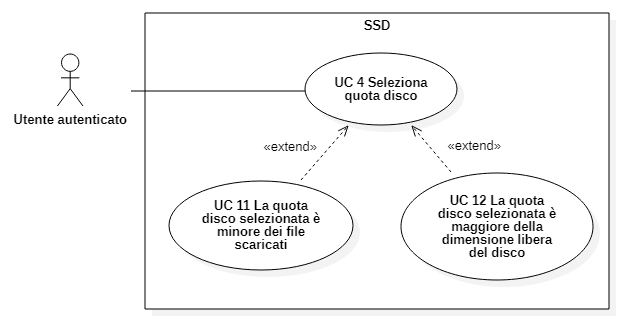
\includegraphics[scale = 0.9]{components/img/UC4.png}
    \caption{UC4 - Visualizzazione messaggio di errore}
\end{figure}
\begin{itemize}
\item \textbf{Attore Primario:} Utente autenticato;
\item \textbf{Precondizione:} Il sistema rileva una condizione di errore;
\item \textbf{Postcondizione:} Viene mostrato un messaggio di errore opportuno;
\item \textbf{Scenario principale:}
    \begin{enumerate}
    \item Il sistema rileva una condizione di errore e mostra un messaggio di errore relativo al contesto nel quale si è riscontrata l'anomalia.
    \end{enumerate}
\end{itemize}